% THIS IS SIGPROC-SP.TEX - VERSION 3.1
% WORKS WITH V3.2SP OF ACM_PROC_ARTICLE-SP.CLS
% APRIL 2009
%
% It is an example file showing how to use the 'acm_proc_article-sp.cls' V3.2SP
% LaTeX2e document class file for Conference Proceedings submissions.
% ----------------------------------------------------------------------------------------------------------------
% This .tex file (and associated .cls V3.2SP) *DOES NOT* produce:
%       1) The Permission Statement
%       2) The Conference (location) Info information
%       3) The Copyright Line with ACM data
%       4) Page numbering
% ---------------------------------------------------------------------------------------------------------------
% It is an example which *does* use the .bib file (from which the .bbl file
% is produced).
% REMEMBER HOWEVER: After having produced the .bbl file,
% and prior to final submission,
% you need to 'insert'  your .bbl file into your source .tex file so as to provide
% ONE 'self-contained' source file.
%
% Questions regarding SIGS should be sent to
% Adrienne Griscti ---> griscti@acm.org
%
% Questions/suggestions regarding the guidelines, .tex and .cls files, etc. to
% Gerald Murray ---> murray@hq.acm.org
%
% For tracking purposes - this is V3.1SP - APRIL 2009

\documentclass{acm_proc_article-sp}

\usepackage[colorlinks=true,linkcolor=blue]{hyperref}	% For hyper links
\usepackage{caption}
\usepackage{subcaption}

\usepackage{fontspec} 
\usepackage{xeCJK}
\setCJKmainfont{BiauKai}

%\usepackage{polyglossia}
%\setmainlanguage{english}
%\setotherlanguage{arabic}
%\newfontfamily\arabicfont{Scheherazade}

\graphicspath{ {./Figures/} }

\begin{document}

\title{Bootstrapping Language-Agnostic Event Detection in Social Media Streams with Sporting Events}
%
% You need the command \numberofauthors to handle the 'placement
% and alignment' of the authors beneath the title.
%
% For aesthetic reasons, we recommend 'three authors at a time'
% i.e. three 'name/affiliation blocks' be placed beneath the title.
%
% NOTE: You are NOT restricted in how many 'rows' of
% "name/affiliations" may appear. We just ask that you restrict
% the number of 'columns' to three.
%
% Because of the available 'opening page real-estate'
% we ask you to refrain from putting more than six authors
% (two rows with three columns) beneath the article title.
% More than six makes the first-page appear very cluttered indeed.
%
% Use the \alignauthor commands to handle the names
% and affiliations for an 'aesthetic maximum' of six authors.
% Add names, affiliations, addresses for
% the seventh etc. author(s) as the argument for the
% \additionalauthors command.
% These 'additional authors' will be output/set for you
% without further effort on your part as the last section in
% the body of your article BEFORE References or any Appendices.

\numberofauthors{3} %  in this sample file, there are a *total*
% of EIGHT authors. SIX appear on the 'first-page' (for formatting
% reasons) and the remaining two appear in the \additionalauthors section.
%
\author{
% You can go ahead and credit any number of authors here,
% e.g. one 'row of three' or two rows (consisting of one row of three
% and a second row of one, two or three).
%
% The command \alignauthor (no curly braces needed) should
% precede each author name, affiliation/snail-mail address and
% e-mail address. Additionally, tag each line of
% affiliation/address with \affaddr, and tag the
% e-mail address with \email.
%
% 1st. author
\alignauthor
Cody Buntain\\
       \affaddr{Dept. of Computer Science}\\
       \affaddr{University of Maryland}\\
       \affaddr{College Park, Maryland 20742}\\
       \email{cbuntain@cs.umd.edu}
% 2nd. author
\alignauthor
Jimmy Lin\\
       \affaddr{College of Information Studies}\\
       \affaddr{University of Maryland}\\
       \affaddr{College Park, Maryland 20742}\\
       \email{jimmylin@cs.umd.edu}
\alignauthor
Jen Golbeck\\
       \affaddr{College of Information Studies}\\
       \affaddr{University of Maryland}\\
       \affaddr{College Park, Maryland 20742}\\
       \email{golbeck@cs.umd.edu}
% Just remember to make sure that the TOTAL number of authors
% is the number that will appear on the first page PLUS the
% number that will appear in the \additionalauthors section.
}

\maketitle
\begin{abstract}
{\color{red}
Lorem ipsum dolor sit amet, consectetur adipiscing elit. Etiam tristique quam dolor, sed fermentum eros commodo eget. Nunc sem ante, tempor gravida gravida quis, vehicula nec dui. Integer hendrerit laoreet mi eu commodo. Integer lacus metus, suscipit at dignissim eget, blandit eget velit. Aenean ac porta metus, ac ultrices sem. Integer tincidunt arcu tortor, id sollicitudin lorem finibus nec. Morbi dignissim purus eget est porta interdum. Nulla faucibus lacinia dignissim. Praesent at nibh dignissim, placerat arcu sit amet, interdum orci.

In volutpat gravida turpis, nec ornare quam. Nam elementum elit non risus rhoncus, facilisis feugiat massa commodo. Vestibulum tempor felis et porttitor vestibulum. Nullam odio neque, ornare in interdum vel, volutpat quis ipsum. Integer vel finibus erat. Quisque eu mi vehicula erat imperdiet vestibulum. Sed laoreet eros lacinia aliquam mollis. Donec fringilla ante id ex pellentesque ultrices. Interdum et malesuada fames ac ante ipsum primis in faucibus.
}
\end{abstract}

% A category with the (minimum) three required fields
\category{H.2.8}{Database Applications}{Data Mining}
\category{\\H.3.3}{Information Search and Retrieval}{Information Filtering}

\keywords{event detection, twitter, social networks, temporal features}

%\keywords{ACM proceedings, \LaTeX, text tagging} % NOT required for Proceedings

\section{Introduction}

Social media's recent ubiquity has drastically altered the velocity with which we spread and consume information, transforming how news and opinions propagate across the planet. 
This democratization of information dissemination has both researchers and traditional media organizations considering social media as a viable complement or alternative to real-time news sources.
For instance, existing research demonstrates social media sources can perform on par with existing newswire sources for certain types of breaking news stories \cite{petrovic2013can}.
While such social media-based systems are able to detect noteworthy events rapidly and in near real time, they often come with restrictive assumptions to facilitate the event-detection task by requiring a priori knowledge of event types, limited target languages, pre-specified event-centric queries, and preprocessing with expensive language models.
Resulting systems are brittle and inflexible in application and are difficult to adapt to new domains, languages, or events.
Forgoing these simplifying restrictions and processing an unfiltered social media stream is a more difficult task, but advantages like multi-language event detection and novel/unexpected event discovery have many practical and important applications that are unsatisfied by current technology.

An alternative avenue for this unfiltered event detection task is to disregard the semantics of the data and focus on the temporal patterns that comprise breaking news and high-impact events.
Given the ``unreasonable effectiveness of data'' and the shear volume of social media content  generated per minute (hundreds of thousands of comments, statuses, and photos on Facebook alone as of 2012 \cite{Pring2012}), it is possible that usage patterns alone could provide interesting cues for detecting events without relying on linguistic understanding and the drawbacks such a reliance necessitates.
Existing work already achieves acceptable performance in detecting events within social media streams when event types and keywords are known before hand, but what if we could achieve the same level of performance in a language-agnostic way and without the need to specify keywords up front?

To explore these questions, we propose a method for learning bursty patterns in the Twitter stream in response to key events in large sporting competitions and using the frequencies of tokens exhibiting such bursts to detect new events of interest.
Sporting events are of particular interest here because they are both highly followed and occur regularly but also include unpredictable patterns of events around points scored, fouls committed, and other occurrences of high interest to followers.
Our experiments on a number of sporting competitions demonstrate how our language-agnostic, frequency-based technique performs comparable to targeted, keyword-centric methods while simultaneously providing additional insight across languages and without requiring expensive text normalization.

\section{Related Work}

{\color{red}
With social media's explosive popularity and the ease with which users can post information using a variety of means (mobile applications, the Web, or via text message), the huge volumes of data now being published has proven useful for a variety of purposes, the most popular of which concentrates on event detection and summarization.
In 2009, researchers began transferring expertise on event detection from traditional news and blog data to social network-based microblogs like Twitter.
Nagarajan et al. adapted existing spatio-temporal analysis to their Twitris framework to identify and localize specific themes according to region \cite{Nagarajan:2009:SAC:1692411.1692481}.
Twitris relies on Google's ``Insights for Search'' to identify trending keywords for a given location or time interval; these keywords are fed into Twitter's search API to bootstrap data collection.
Twitris clusters these trending tokens to identify thematically similar content and present groups of related tokens as retrospective event ``storylines.''
Though Twitris and similar systems \cite{Sankaranarayanan:2009:TNT:1653771.1653781,Long:2011:TEE:2035562.2035636} are powerful, their event summaries are too coarse to detect individual occurrences in sports and rely heavily on traditional media to bootstrap the detection process.

Cataldi et al. take a different approach in their 2010 paper on detecting emerging topics in Twitter by leveraging ``user authority'' as calculated using the well-known Google PageRank algorithm \cite{Cataldi:2010:ETD:1814245.1814249}.
Though this approach might be useful for identifying authoritative sources like sports journalists or official team Twitter accounts, our approach forgoes user characteristics.
Instead, we prioritize token-centric burst information over  a user's network influence since only a limited number of fans tweeting about some event may be authoritative in the network.

Work by Petrovi\'{c}, Osborne, et al. is perhaps the most similar system to ours \cite{Petrovic:2010:SFS:1857999.1858020,petrovic2013can,osborne2014real}.
This system, called ReDites, relies on locality sensitive hashing (LSH) to enable near real-time tweet clustering for event detection but is restricted to only for English-language tweets.
LSH allows for fast similarity calculations to determine a message's ``nearest neighbor,'' which enables high-speed clustering for theme/event generation.
Once ReDites constructs these themes, it can perform a retrospective analysis to identify the first story related to a given theme.
Our approach has a language flexibility that ReDites lacks, and we focus more on identifying events as they occur rather than retrospectively, but ReDites's ability to handle many Twitter messages at an extremely high rate is an impressive benchmark for which we are striving for future versions.

Only recently has event detection specific to sports gathered more attention.
Lanagan and Smeaton tried to align changes in tweet volume of a filtered Twitter stream with an annotated audio/video analysis and showed that bursts in Twitter usage co-occurred with high-impact events\cite{lanagan2011using}.
Zhao et al. used a lexicon of American football-related terms to refine the Twitter stream and detect events during the 2010-2011 NFL football season within 40 seconds \cite{Zhao2011}.
Vasudevan et al. used Twitter to identify events specific to American football and found that events could be detected within a few minutes of the actual event \cite{vasudevan2013twitter}.
The common threads among all these approaches, however, are prior knowledge of event type and a pre-specified set of event keywords, which limits their applicability to international sports and other languages.
}

\section{Methodology}

This paper's primary goal is to demonstrate how our language-agnostic technique is able to detect significant events in sporting competitions as accurately as the baseline known target token method.
While our method requires no input regarding event type, the baseline accepts a set of keywords related to specific events of interest; since we focus on the sporting domain, these tokens might include ``goal,'' ``score,'' ``card,'' ``foul,'' or similar keywords that relate to interesting events.
After training our method on a number of sporting events from the past five years, we use existing metrics to compare event detection performance in the 2013 World Series, 2014 Super Bowl, and 2014 World Cup.
The remainder of this section presents the details of both our language-agnostic approach and the baseline technique before describing the overall experimental framework we used for comparison.

\subsection{Data Collection and Sporting Events}

Though this work is general in nature, much of the development leverages the Twitter social network since a large amount of research on this network exists, and data is relatively easy to acquire.
Specifically, this research leveraged three separate Twitter data sources: an excerpt from the Edinburgh Twitter Corpus \cite{Petrovic:2010:ETC:1860667.1860680}, a selection of tweets from the Twitter Firehose covering Argentina in November of 2011, and various days in 2013 and 2014 from the Twitter 1\% sample garden hose.

To model bursty tokens across a wide variety of sporting events, we first needed ground truth with known tokens and timestamps that correspond to actual events within sporting competitions.
We reviewed our collections of Twitter data and generated a series of timestamped events and related tokens for thirteen different sporting events: 

\begin{itemize}
\item The 2010 National Football Championship game, 
\item Four premier league soccer games in November of 2012, %(Arsenal de Sarand\`{i} versus V\'{e}lez Sarsfield on November 3, Barcelona versus Mallorca on November 11, Argentina versus Saudi Arabia on November 14, and Argentina versus Brazil on November 22), 
\item The final two games of the 2013 Major League Baseball (MLB) World Series, 
\item The National Football League's (NFL) 2014 Super Bowl, 
\item The National Hockey League's (NHL) 2014 playoffs, 
\item The National Basketball Association's (NBA) 2014 playoffs, 
\item The 2014 Kentucky Derby, 
\item The 2014 Belmont Stakes, 
\item And a selection of games from the 2014 F\'{e}d\'{e}ration Internationale de Football Association (FIFA) World Cup.
\end{itemize}

For each event, we used existing blog posts, news articles, and social media data to construct timelines for in-game events like scores, fumbles, and penalties, which were used as positive samples.
For negative samples to differentiate between bursty and non-bursty tokens, it is difficult to acquire negative samples since we cannot know \emph{all} tokens that should be bursting on Twitter at a specific time.
We can, however, assume that stop words should never experience bursts in usage; as such, we naively tagged English and Spanish stop words as negative samples.

\subsection{Experimental Framework}

We compared our language-agnostic classifier with the target-token frequency baseline on identifying four types of events: scores, penalties, game starts, and game ends.
Evaluation used a test set comprised of the final two games of the 2013 MLB World Series, the 2014 NFL Super Bowl, and the 2014 FIFA World Cup.
For the World Series, this set contained the final two games on 28 October and 30 October of 2013, between the Boston Red Sox and the St. Louis Cardinals, which contained four events of game starts/ends and ten instances of points scored.
The 2014 Super Bowl occurred on 2 February 2014 and contained a game start, an end, and also ten instances of points scored.
Our World Cup data covered the final two matches on 12 July and 13 July 2014 between the Netherlands and Brazil and Germany and Argentina respectively.
Between these two matches, we had four game starts/ends, nine penalty cards issued, and four goals scored.

For each approach described herein, we generate receiver operating characteristic (ROC) curves across each sport and then a combined ROC curve for all sports and compare the area under the curves for both methods.

\subsection{Language-Agnostic Event Detection}

As mentioned, existing research achieves acceptable performance in event detection by tracking frequencies for a small set of keywords that should experience bursts in usage when a real-world event occurs (e.g., ``goal'' should experience a burst when a player scores a goal in soccer/football).
Rather than rely on these known tokens directly, we built a collection of such tokens across several sporting events and sports types and constructed a set of temporal features to model bursts.
In each collection, we filter out messages flagged as retweets and disregard hashtags.
These temporal features were built around a sliding window of several minutes with each window further divided into overlapping slices to construct a time series for each token.
Feature vectors generated for each bursty token taken with those vectors from a set of known stop words allowed us to cast this bursty modeling task as a machine learning problem to delineate between bursting and non-bursting tokens.
Finally, applying a threshold to the number of tokens classified as bursting per window allowed us to identify those windows in which significant real-world events occurred and supported extracting tokens that described those events.
Each of these steps is detailed more thoroughly below.

\subsubsection{Temporal Features}

While previous work already covers burst detection, only a subset is relevant to the streaming case presented herein, and we integrated those into our system.
Beyond these existing features, we also developed a number of features that should yield higher weights for tokens that deviate significantly from normal posting frequencies:

\begin{itemize}
\item \textbf{Frequency Regression} Given the log of a token's frequency at each slice in the current window, take the slope of the best-fitting line.
\item \textbf{Message Frequency Regression} Given the log of the number of tweets in which a token appears for each slice in the current window, take the slope of the best-fitting line.
\item \textbf{User Frequency Regression} Given the log of the number of users using a token at each slice in the current window, take the slope of the best-fitting line.
\item \textbf{Average Frequency Difference} The difference between the token's frequency in the most recent slice and the average frequency across the current window.
\item \textbf{Message Average Frequency Difference} The difference between the number of messages in which a token appears in the most recent slice and the average number of messages containing that token across the current window.
\item \textbf{User Average Frequency Difference} The difference between the number of users who use a token in the most recent slice and the average number of users across the current window.
\item \textbf{Inter-Arrival Time} The average number of seconds between token occurrences in the given window.
\item \textbf{Entropy} The entropy of the set of tweets containing a given token.
\item \textbf{TF-IDF} The term frequency, inverse document frequency for a each token.
\item \textbf{TF-PDF} A modified version of TF-IDF called term frequency, proportional document frequency \cite{Bun:2002:TEN:645962.674082}.
\item \textbf{BursT} Weight using a combination of a given token's actual frequency and expected token frequency \cite{Lee:2011:BDT:2009463.2009531}.
\end{itemize}

We normalized feature vectors into the range $[0, 1]$ to avoid biases from scale during classification by taking the maximum and minimum values for each feature in the current window.

\subsubsection{Training the Ensemble Classifier}

Discriminating between bursty tokens and stop words necessitated the use of a classification algorithm, and many different such algorithms exist.
In particular, the Scikit-learn Python package provides implementations for support vector machines (SVMs) and random forests (RFs) as well as an implementation of the ensemble classifier AdaBoost \cite{scikit-learn}.
Both SVMs and RFs have tunable parameters to select before integrating into AdaBoost, however, so we developed a grid search strategy to select parameters based on the F1 scores on our training and testing data.

For SVMs, we used the radial basis kernel, which has two parameters: cost $c$ and kernel coefficient $\gamma$.
In searching the space of $c$ and $\gamma$, the grid covered powers of two such that $c = 2^x$, $x \in [-2, 10]$ and $\gamma = 2^y$, $y \in [-2, 5]$.
For each pair of parameter values, we trained thirty different classifiers using repeated random subsampling, took the average F1 score, and selected the parameter set with the highest F1 score.
Selecting parameter values for RFs was similar for the number of estimators $n$ and feature count $c'$ such that $n = 2^x$, $x \in [0, 10]$ and $c' = 2^y$, $y \in [1, 11]$.
This training procedure yielded the results shown in Table \ref{tab:scores}.

\begin{table}[htdp]
\caption{Classifier Parameter Scores}
\begin{center}
\begin{tabular}{|c|c|c|c|c|}
\hline
\textbf{Classifier} & \textbf{Params} & \textbf{F1-Score} \\ \hline
SVM & $c=64,$ & 0.588410 \\ 
& $\gamma=4$ & \\ \hline
RF & trees = 128, & 0.575301 \\
& features = 9 &  \\ \hline
\end{tabular}
\end{center}
\label{tab:scores}
\end{table}

These two classifiers were then combined using the Scikit-learn's AdaBoost implementation with four estimators.
We then applied the resulting AdaBoost classifier to all the training data and expanded our set of known bursty tokens with those tokens that had a greater than 90\% likelihood of being part of the bursty class in one round of self-training (Scikit's AdaBoost implementation provides likelihoods for tokens it predicts).

Regarding sliding window and slice size, preliminary investigations seemed to illustrate a window size of ten minutes with a slice size of three minutes (each slice overlapped the next by two minutes) lead to acceptable results.

\subsection{Baseline Event Detection}

Inspired by existing work on event detection like that from Twitter's blog on detecting goals during the World Cup, the baseline we developed takes as input a set of keywords that should exhibit bursts in usage during related events, performs some rudimentary normalization to collapse modified words down to their originals (e.g., ``goooooooaaaallll'' down to ``goal''), and uses a sliding window to compare the current frequency of those keywords to their average frequency \cite{Cipriani2014}.
If the frequency in the current window exceeds some threshold, which is set as some multiple of the average, we say an event was detected in that window.
As with the language-agnostic method, we used a sliding window of ten minutes as well.

Since our analysis covers three separate types of sporting competitions, the keyword list for this method must include tokens from the vocabulary of each. 
We avoid separate keyword lists for each sport to provide a more even comparison to the general nature of our language-agnostic technique.

The keywords for which we searched were as follows: ``goal'', ``gol'', ``golazo'', ``score'', ``foul'', ``penalty'', ``card'', ``red'', ``yellow'', ``touchdown'', ``td'', ``fieldgoal'', ``points'', ``run'', ``home'', ``homerun''.
Additionally, the following regular expressions collapsed deliberately misspelled tokens down to their normal counterparts: ``g+o+a+l+'' $\rightarrow$``goal'', ``g+o+l+'' $\rightarrow$``gol'', ``g+o+l+a+z+o+'' $\rightarrow$``golazo'', ``sco+red?'' $\rightarrow$``score''.

\section{Results}

To restate, the research question posed in this work is to determine whether a language-agnostic, streaming event detection scheme can perform as well as a domain-specific frequency-based method in detecting events in sporting competitions.
We answer this question across three separate sporting events: the final two games of the 2013 MLB World Series, the 2014 NFL Super Bowl, and the final two matches of the 2014 FIFA World Cup.

For each event, we generated ROC curves by varying a threshold parameter and calculating the true and false positive rates.
In the baseline, pre-specified token approach, our threshold parameter varied the difference between the current frequency sum of the target keywords.
For our language-agnostic, bursty method (``LA Bursty'' in the figures) , the ROC curve was generated by varying the minimum number of tweets a window must contain for an event to be detected.
We then compared the area under the curve (AUC) metric to determine the difference in performance between the two methods.
Prior to presenting comprehensive results, we first present performance curves for each event type.

\subsection{2013 World Series}

For the 2013 World Series, the two tested techniques exhibited similar performance, with a difference of only 0.02 (the baseline with 0.76 and the language-agnostic bursty method with 0.74).
Figure \ref{fig:roc2013WorldSeries} shows the how these two curves compare graphically, and we can see that neither curve truly dominates the other, and both perform better than random guessing.

\begin{figure}[hbtp]
\begin{center}
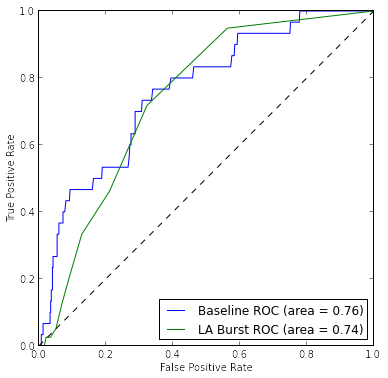
\includegraphics[width=3.25in]{./figures/roc_2013_WorldSeries.png}
\caption{ROC Curves for the 2013 World Series}
\label{fig:roc2013WorldSeries}
\end{center}
\end{figure}

\subsection{2014 Super Bowl}

For the 2013 World Series, the two tested techniques exhibited similar performance, with a difference of only 0.02 (the baseline with 0.76 and the language-agnostic bursty method with 0.74).
Figure \ref{fig:roc2014SuperBowl} shows the how these two curves compare graphically, and we can see that neither curve truly dominates the other, and both perform better than random guessing.

\begin{figure}[hbtp]
\begin{center}
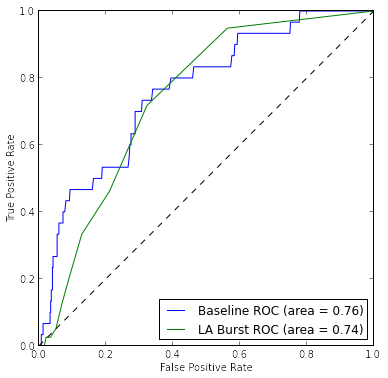
\includegraphics[width=3.25in]{./figures/roc_2013_WorldSeries.png}
\caption{ROC Curves for the 2014 Super Bowl}
\label{fig:roc2014SuperBowl}
\end{center}
\end{figure}

\subsection{2014 World Cup}

For the 2013 World Series, the two tested techniques exhibited similar performance, with a difference of only 0.02 (the baseline with 0.76 and the language-agnostic bursty method with 0.74).
Figure \ref{fig:roc2014WorldCup} shows the how these two curves compare graphically, and we can see that neither curve truly dominates the other, and both perform better than random guessing.

\begin{figure}[hbtp]
\begin{center}
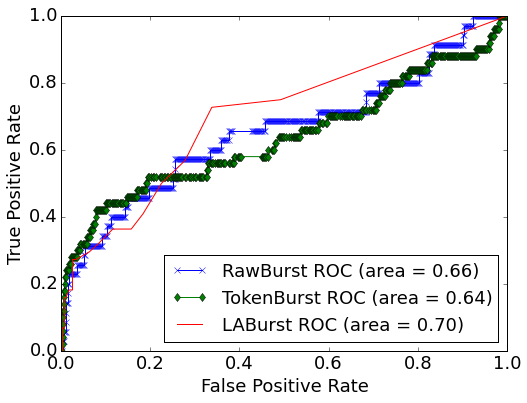
\includegraphics[width=3.25in]{./figures/roc_2014_WorldCup.png}
\caption{ROC Curves for the 2014 World Cup}
\label{fig:roc2014WorldCup}
\end{center}
\end{figure}

\subsection{Composite Results}

To compare comprehensive performance, we look to Figure \ref{fig:rocComprehensive}, which shows ROC curves for both methods across all three event types.
From this figure, we see the two methods perform nearly identically with AUC values of 0.7187 for the baseline and 0.7052 for our language-agnostic technique.
Assuming equal cost for false positives and false negatives and optimizing for the largest difference between true positive rate (TPR) and false positive rate (FPR), the baseline method shows 0.5581 and 0.1408 respectively with a difference of 0.4174 at a threshold value of 13.2.
Our language-agnostic method, on the other hand, has a TPR of 0.7105 and FPR of 0.3518 with a difference of 0.3587 at a threshold value of 2.
From these values, we see our approach achieves a higher true positive rate but at a cost of a higher false positive rate as a result.

\begin{figure*}[hbtp]
\begin{center}
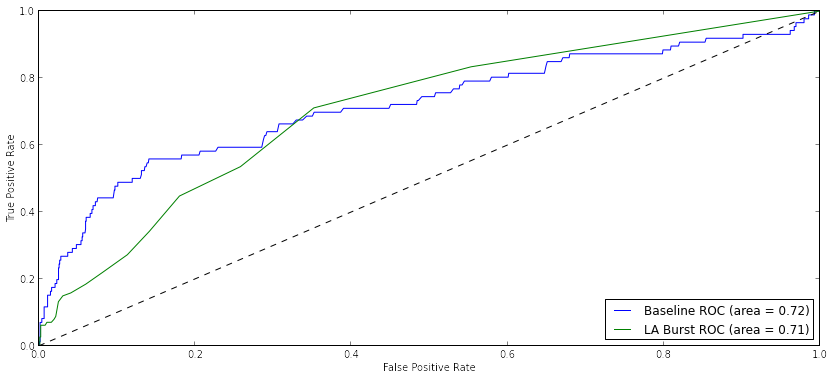
\includegraphics[width=6in]{./figures/roc_Comp.png}
\caption{Composite ROC Curves}
\label{fig:rocComprehensive}
\end{center}
\end{figure*}

\subsection{Earthquake Detection}

Detecting sub-events within sporting competitions as described above is a useful task for areas like advertising or automated highlight generation, but a more interesting and worthwhile task would be to detect higher-impact events like natural disasters.
The typical frequency-based approach is more difficult here as it is impossible to know what events are about to happen, and a list of target keywords to detect all such events would be long, leading to false positives.
Our method could be highly beneficial here as one would not need to know the target language or other pre-specified information.
Since Sakaki showed the feasibility of detecting earthquakes using Twitter, we pulled Twitter data for two earthquakes in Japan: a 7.1-magnitude quake off the coast of Honshu on 25 October 2013, and a 6.5-magnitude quake off the coast of Iwaki on 11 July 2014.

To determine whether our approach could detect these earthquake events, we applied the classifier trained and tested for the sporting domain to these Twitter sets and tracked the frequency of the term ``earthquake'' simultaneously.
Figures \ref{fig:2013Japan} and \ref{fig:2014Japan} show the frequencies for both methods for the 2013 and 2014 earthquakes respectively; the red dots indicate the earthquake times as reported by the United States Geological Survey (USGS).
From these figures, one can see the token ``earthquake'' sees a significant increase in usage when the earthquake occurs, and our language-agnostic method experiences a similar increase at the same moment for both events.
That is, both techniques identify the earthquake simultaneously.

\begin{figure}[hbt]
\begin{center}
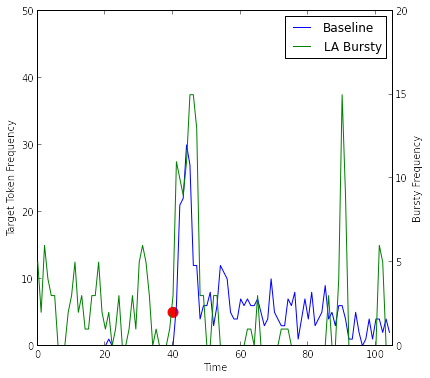
\includegraphics[width=3in]{./figures/2013-japan-quake.png}
\caption{Honshu, Japan Earthquake - 25 October 2013}
\label{fig:2013Japan}
\end{center}
\end{figure}

\begin{figure}[hbtp]
\begin{center}
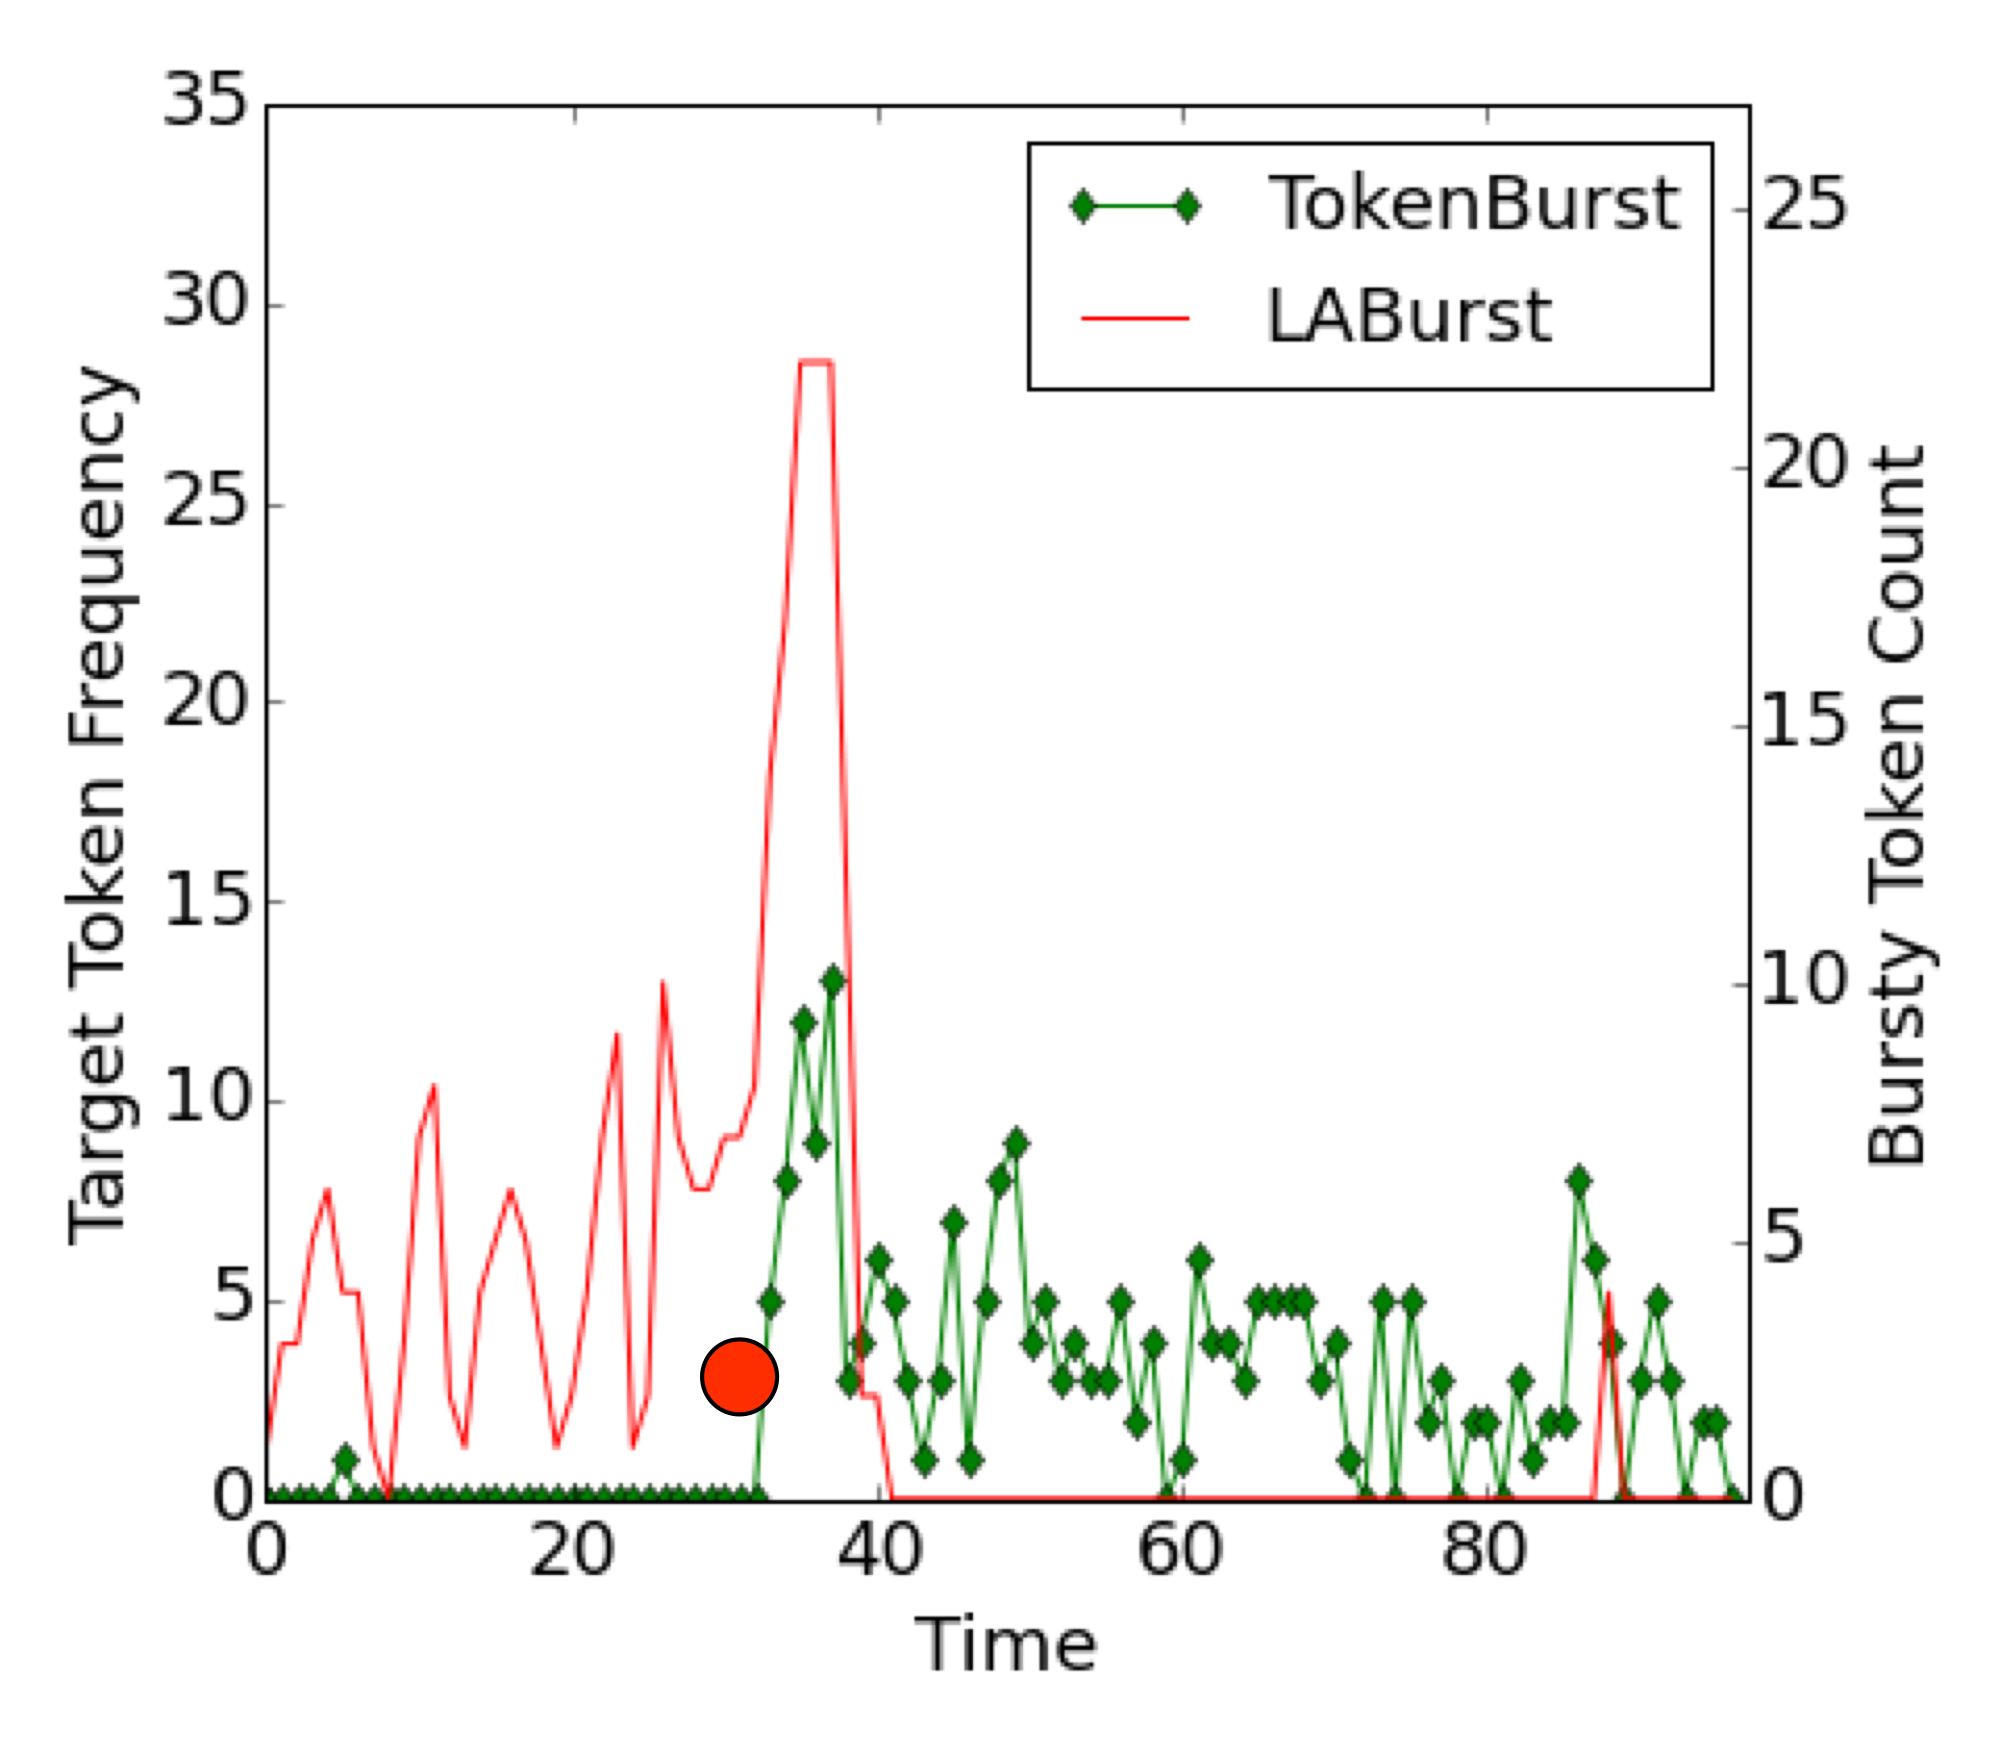
\includegraphics[width=3in]{./figures/2014-japan-quake.png}
\caption{Iwaki, Japan Earthquake - 11 July 2014}
\label{fig:2014Japan}
\end{center}
\end{figure}

Given our method's success here, one can now ask what tokens we identified as bursting when the earthquakes occurred.
Many of the tokens are in Japanese, and tokens at the peak of the earthquake events are shown in Table \ref{tab:japanTokens}.
We also extracted tweets from our data that contain the highest number of these tokens for the given time period, a selection of which include, ``地震だあああああああああああああああああああああ,'' ``今回はチート使ってないから地震わからなかった,'' and ``地震だー.''
Google Translate\footnote{http://translate.google.com} translates these tweets as ``Ah ah ah ah ah ah ah ah ah Aa's earthquake,'' ``I did not know earthquake because not using cheat this time,'' and ``Over's earthquake'' respectively.

\begin{table}[htdp]
\caption{Tokens Classified as Busting During Events}
\begin{center}
\begin{tabular}{|p{1.45in} | p{1.45in} |}
\hline
\multicolumn{1}{|c|}{\textbf{Match}} & \multicolumn{1}{|c|}{\textbf{Bursty Tokens}} \\ \hline
Honshu, Japan -- 25 October 2013 & \c{c}dostum, 丈, 地, 報, 夫, 島, 怖, 揺, 構, 波, 注, 津, 源, 福, 長, 震 \\ \hline
Iwaki, Japan -- 11 July 2014 & antojo, comida, sammy, び, ゆ, ビビ, 地, 報, 島, 怖, 急, 福, 緊, 臓, 警, 速, 震 \\ \hline
\end{tabular}
\end{center}
\label{tab:japanTokens}
\end{table}

\section{Analysis}

In comparing the baseline and language-agnostic techniques, it is important to understand the baseline provides little in the way of discovering previously unknown tokens or significant events that do not conform to a priori knowledge.
The real power of the language-agnostic method described herein addresses such deficiencies directly by identifying specific tokens that burst along with a significant event \emph{and} by capturing unexpected events.

\subsection{Identifying Event-Related Tokens}

As mentioned, where the baseline requires the user to specify interesting or event-related tokens prior to any data processing or analysis, our approach identifies these event-related tokens automatically.
These tokens may include misspellings, colloquialisms, and cross language boundaries, which makes them hard to know before hand.
The 2014 World Cup presents an interesting case for finding these otherwise unexpected tokens because the event has enormous international viewership; as such, many Twitter users of many different languages are likely tweeting about the same event.

To explore the tokens generated during these high-profile events, we look to those tokens identified as bursting during several events in the final two World Cup matches.
Table \ref{tab:burstyTokens} shows a selection of events from these matches and a subset of those tokens classified as bursting during the events (one should note the list is not exhaustive owing to formatting and space constraints).

\begin{table}[htdp]
\caption{Tokens Classified as Busting During Events}
\begin{center}
\begin{tabular}{|p{0.75in}|p{0.7in}| p{1.45in} |}
\hline
\multicolumn{1}{|c|}{\textbf{Match}} & \multicolumn{1}{|c|}{\textbf{Event}} & \multicolumn{1}{|c|}{\textbf{Bursty Tokens}} \\ \hline
Brazil v. Netherlands, 12 July 2014 & Netherlands' Van Persie scores a goal on a penalty at 3', 1-0 & 0-1, 1-0, 1:0, 1x0, card, goaaaaaaal, goal, gol, goool, holandaaaa, k\i{}rm\i{}z\i{}, pen, penal, penalti, p\^{e}nalti, persie, red \\ \hline
Brazil v. Netherlands, 12 July 2014 & Brazil's Oscar get's a yellow card at 68' & dive, juiz, penalty, ref \\ \hline
Germany v. Argentina, 13 July 2014 & Germany's G\"{o}tze scores a goal at 113', 1-0 & goaaaaallllllll, goalllll, godammit, goetze, gollllll, gooooool, gotze, gotzeeee, g\"{o}tze, nooo, yessss, ドイツ, لااااااا \\ \hline
\end{tabular}
\end{center}
\label{tab:burstyTokens}
\end{table}

Several interesting artifacts emerge from this table, first of which is that one can get an immediate sense of the detected event from tokens our algorithm presents. 
For instance, the prevalence of the token ``goal'' and its variations clearly indicate a team scored in the first and third events in Table \ref{tab:burstyTokens}; similarly, bursting tokens associated with the middle event regarding Oscar's yellow card reflect his penalty for diving.
Beyond the pseudo event description put forth by the identified tokens, this reference to diving and to specific player and teams names in the first and third events are also of significant interest.
In the first event, one can infer that the Netherlands scored since ``holandaaaa'' is flagged along with ``persie'' from the Netherlands' player Van Persie, and likewise for Germany's G\"{o}tze in the third event (and the accompanying variations of his name).
These terms would be difficult to capture beforehand as would be required in the baseline and would likely not be related to every event or every type of sporting event.

Finally, the last artifact of note is that the set of bursty tokens displayed includes tokens from several different languages: English for ``goal'' and ``penalty,'' Spanish for ``gol'' and ``penal,'' Brazilian Portuguese for ``juiz'' (meaning ``referee''), as well as the Arabic for ``goal'' and Japanese for ``Germany.''
Since these words are semantically similar but syntactically dissimilar, typical normalization schemes could not capture these connections.
Instead, capturing these words in the baseline would require a pre-specific keyword list in all possible languages or the inclusion of an expensive machine translation system that was also capable of normalizing within different languages (to collapse ``goool'' down to ``gol'' for example).

\subsection{Undocumented Event Discovery}

One particular weakness present in the baseline is that it is unable to capture unexpected events or events that do not conform to the keyword list.
This deficiency means analysts might miss significant events within these competitions, especially if they are not directly related to scores or penalties, such as Uruguay's Luis Suarez's biting the Italy's Giorgio Chiellini during a World Cup match on 24 June since no foul was called at the time.
Other instances of particularly dramatic play or events that happen at the larger sporting event but not necessarily on the field might be missed as well.

We can see instances of such omissions in the last game of World Cup.
Figure \ref{fig:worldCupFreqs} shows the frequencies for target tokens for the baseline in blue and bursty tokens for our method in green.
From this graph, we can see the first, obvious incidence in Peak \#1 where our bursty method exhibits a peak that is missed by the baseline in the first few points of data.
The primary tokens appearing in this peak are ``puyol,'' ``gisele,'' and ``bundchen,'' which correspond to former Spanish player Carles Puyol and model Gisele Bundchen, who presented the World Cup trophy prior to the match.
Peak \#2, slightly more than eighty minutes into the data (which is sixty minutes into the match), our burst analysis sees another peak that is otherwise relatively minor in the baseline graph.
Upon further exploration, tokens present in this peak refer to Argentina's substituting in Ag\"{u}ero for Lavezzi at the beginning of the match's second half.

\begin{figure}[hbtp]
\begin{center}
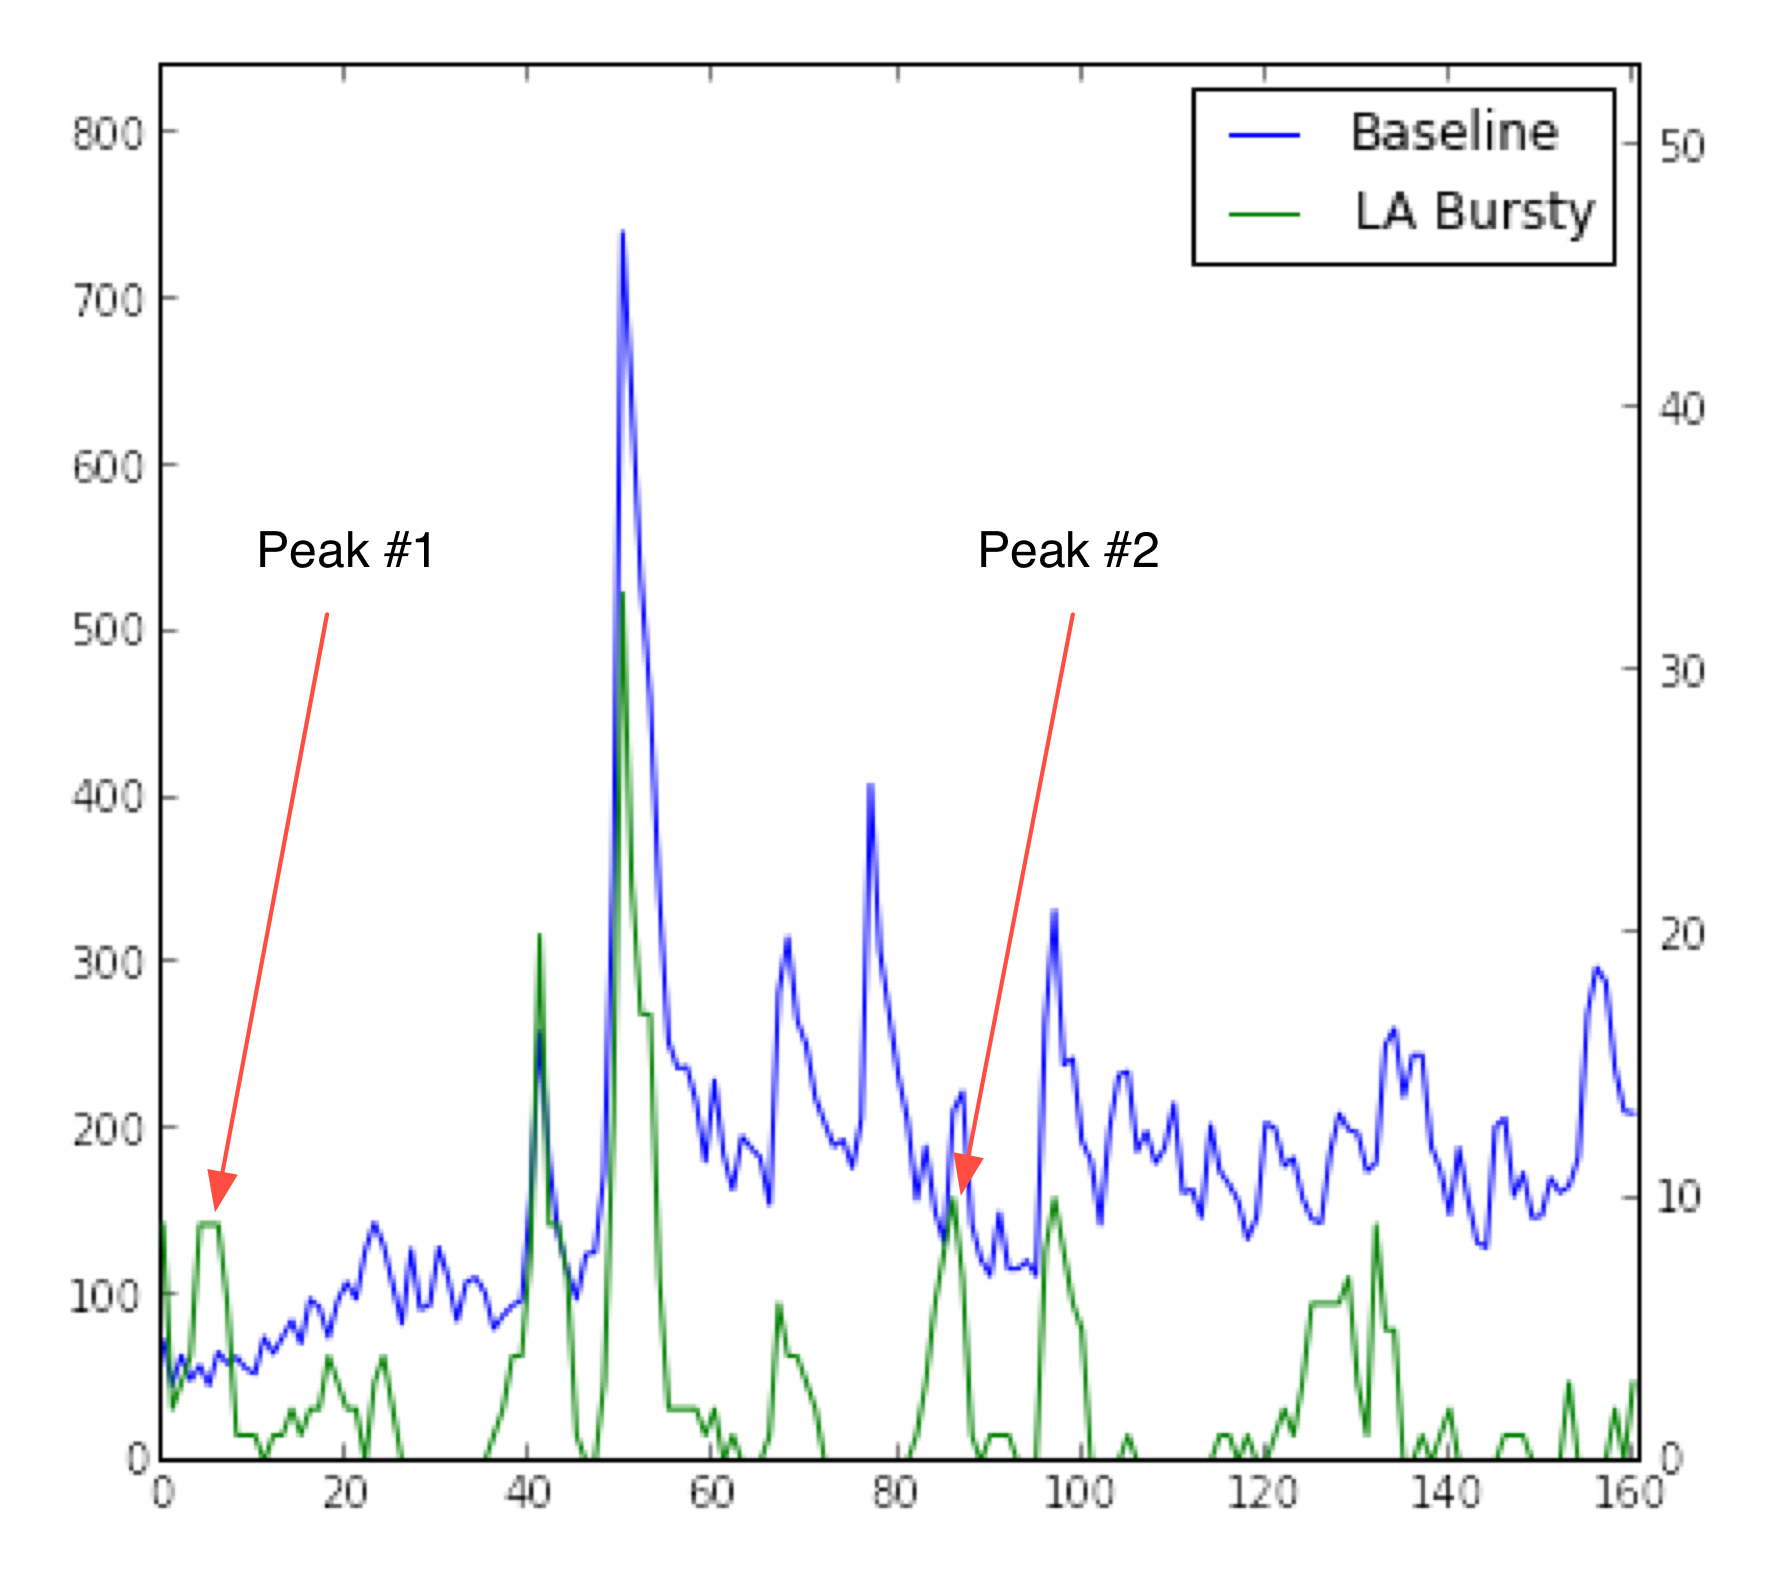
\includegraphics[width=3.25in]{./figures/wc0713freq-labeled.png}
\caption{Baseline and LA Bursty Frequencies}
\label{fig:worldCupFreqs}
\end{center}
\end{figure}

Given our detection of these additional non-score-/non-penalty-related events, it is perhaps unsurprising that our burst detection technique exhibits a higher false-positive rate compared to the baseline.
Since our approach is both language- and domain-agnostic, it makes sense that it would detect additional events beyond the game start/end, score, and penalty events our data counts as ground truth.
A better comparison between the accuracies of the two approaches may be to identify only those peaks in which the keywords used in the baseline are identified as bursty in our method, but such a test disregards our approach's additional power.

\subsection{Real-Time Usage and Event Persistence}

In comparing these two event detection methods, we must also address their abilities to handle streaming data and the lag between an event and its detection by either of these mechanisms.
The baseline technique processes data minute by minute and therefore has at most a minute of lag between input and discovery.
Our technique, on the other hand, exhibits a lag equal to the slice size, which in the case of this paper is three minutes.

Another important aspect to consider is the length of time in which an event's peak persists.
For the baseline, event detection achieves its highest accuracy when events are flagged in the minute they occur and the minute immediately following.
Our approach logically follows the slice length such that events persist for three minutes.

\section{Conclusions}

To revisit our motivations, the goal for this experiment was to demonstrate the feasibility of detecting events and event-related tokens through analyzing temporal characteristics from unfiltered Twitter data streams.
While many social media-based event detection systems require some form of query-based filtering and language model processing, our approach is more flexible, lighter weight, and easily adaptable to different domains.
Our results show that by leveraging temporal characteristics to identify bursty tokens and using frequency of these bursty tokens, we can detect significant events across a collection of disparate sporting competitions with a level of performance nearly equivalent to an existing, domain-specific baseline.

Similar performance to the baseline is only part of the story, however, as our approach offers notable flexibility in identifying bursting tokens without normalization and across language boundaries.
With this versatility also comes support for event description since we no longer rely on predetermined keywords; that is, we can get a sense of the occurring event by inspecting the bursty tokens.
Finally, these advantages culminate in powerful tool for event \emph{discovery} in that it can detect events we did not expect to occur, regardless of the source language, which makes this technique particularly useful for journalists and newswire sources who have a need to know about events on the ground, as they happen but cannot know a priori what the event may be about in all cases.

%\end{document}  % This is where a 'short' article might terminate

%ACKNOWLEDGMENTS are optional
\section{Acknowledgments}
This work made use of the Open Science Data Cloud (OSDC), which is an Open Cloud Consortium (OCC)-sponsored project. 
The OSDC is supported in part by grants from Gordon and Betty Moore Foundation and the National Science Foundation and major contributions from OCC members like the University of Chicago. 
?

%
% The following two commands are all you need in the
% initial runs of your .tex file to
% produce the bibliography for the citations in your paper.
\bibliographystyle{abbrv}
\bibliography{sources}  % sigproc.bib is the name of the Bibliography in this case
% You must have a proper ".bib" file
%  and remember to run:
% latex bibtex latex latex
% to resolve all references
%
% ACM needs 'a single self-contained file'!
%
%APPENDICES are optional
%\balancecolumns
\end{document}
